\documentclass[../PianodiProgetto.tex]{subfiles}

\begin{document}
	
	\chapter{Ciclo di sviluppo}
	
	Il modello di ciclo di sviluppo adottato dal gruppo è il \glossario{modello incrementale}{modello incrementale}. Le motivazioni che hanno portato alla scelta di questo modello sono:
	\begin{itemize}
		\item Possibilità di suddividere il lavoro in più sottoattività sviluppate in modo parallelo. Questo permette maggior controllo sull’avanzamento del progetto;
		\item Lo sviluppo avviene per incrementi, dove ogni incremento rilascia parte delle funzionalità richieste;
		\item I requisiti vengono suddivisi in livelli di priorità. Quelli a priorità maggiore verranno soddisfatti con i primi incrementi, questo permette più attività di verifica e quindi maggiore stabilità ad ogni iterazione;
		\item I primi incrementi possono essere usati come prototipo per aiutare a definire i requisiti degli incrementi successivi;
		\item Minimizzare i rischi di ritardo rispetto ai tempi stabiliti in quanto i cicli hanno durata breve e sono precedentemente pianificati.
	\end{itemize}
	Alla fine della prima fase si avrà un prototipo funzionante con le implementazioni dei requisiti obbligatori. Tramite incrementi successivi verranno integrate le funzionalità opzionali.
	
	\chapter{Pianificazione}
	
	La pianificazione del lavoro stata costruita sulla base delle scadenze elencate alla sezione 2.5 del seguente documento. In base ad esse, si è suddiviso lo sviluppo in cinque periodi. I periodi scelti sono i seguenti:
	\begin{itemize}
		\item Analisi;
		\item Consolidamento dei requisiti;
		\item Progettazione architetturale;
		\item Progettazione di dettaglio e Codifica;
		\item Validazione e collaudo.
	\end{itemize}

	\section{Analisi}
	Inizia il 07-11-2017 con la formazione del gruppo e termina il 16-01-2018 con la scadenza per la consegna dei documenti relativi alla Revisione dei Requisiti.
	Durante questa attività vengono svolte le seguenti sotto-attività:
	\begin{itemize}
		\item \textbf{Norme di Progetto:} vengono individuate dal gruppo tutte le norme e gli strumenti per il corretto svolgimento del progetto, riportando il tutto nel documento \textit{Norme di Progetto};
		\item \textbf{Studio di Fattibilità:} in questa attività vengono studiati i vari capitolati, analizzando i vari pro e contro, scegliendo quale sviluppare, lo studio fatto viene tradotto in forma scritta nel documento \textit{Studio di Fattibilità};
		\item \textbf{Analisi dei Requisiti:} viene effettuata un'analisi approfondita dei requisiti del capitolato che il gruppo ha deciso di sviluppare, il tutto riportato nel documento \textit{Analisi dei Requisiti};
		\item \textbf{Piano di Progetto:} durante questa attività vengono individuate e pianificate le varie attività da svolgere per la realizzazione del progetto suddividendo le risorse disponibili, tutto ciò viene formalizzato nel documento \textit{Piano di Progetto}; 
		\item \textbf{Piano di Qualifica:} vengono definite le metriche per il prodotto, le quali vengono riportate nel \textit{Piano di Qualifica};
		\item \textbf{Glossario:} viene redatto il documento \textit{Glossario}	contenente tutti i termini tecnici, di dominio, gli acronimi e le parole che necessitano di essere chiarite per migliorare la comprensione dei documenti;
		\item \textbf{Lettera di Presentazione:} viene redatta la \textit{Lettera di Presentazione} per presentare la candidatura del gruppo.	
	\end{itemize}
	
	\subsection{Analisi - Diagramma di Gantt}
	\begin{figure}[H]
		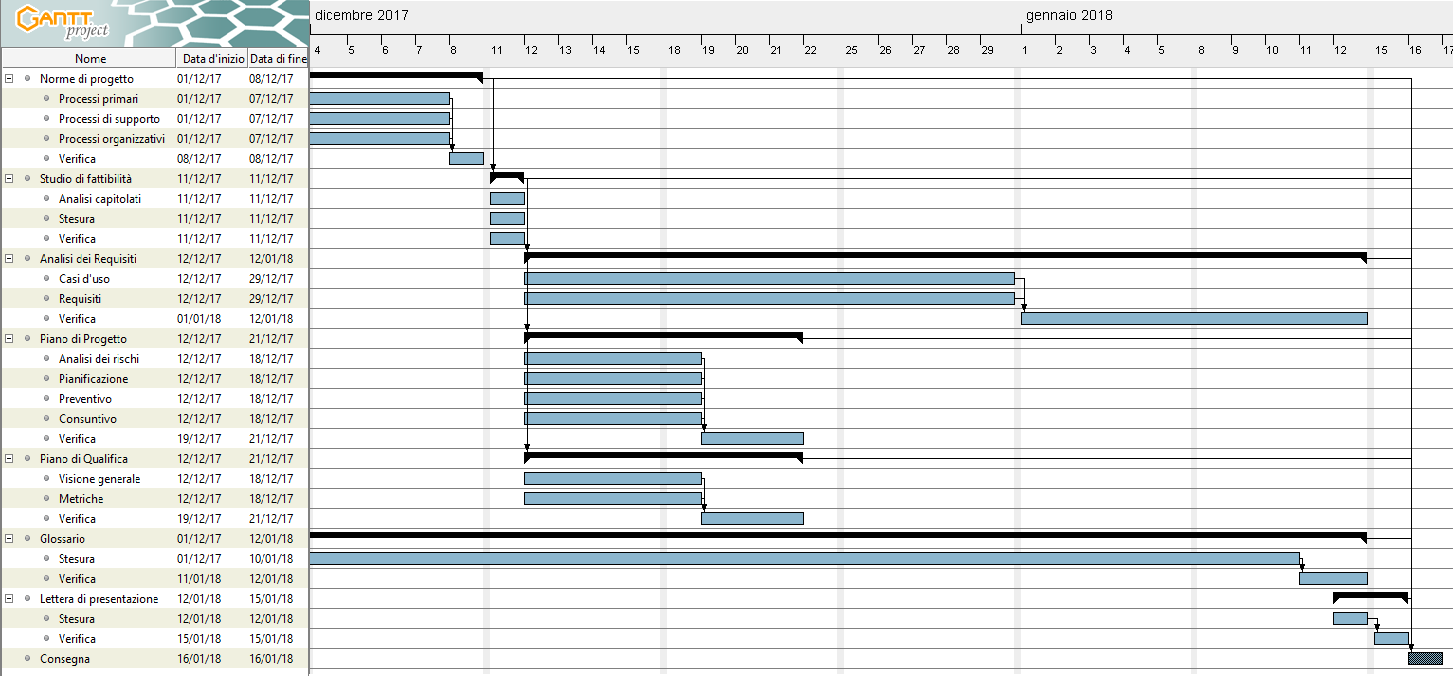
\includegraphics[width=1\linewidth]{AnalisiGantt.png}	
		\caption{Diagramma di Gantt di Analisi}\label{fig:1}	
	\end{figure}
	\newpage
	\section{Consolidamento dei requisiti} Inizia dopo la consegna dei documenti per la Revisione dei Requisiti e termina con la presentazione della Revisione dei Requisiti il 26-01-2018. Questa attività consiste nel migliorare e consolidare quanto fatto nell'Analisi dei Requisiti.
	\subsection{Consolidamento dei requisiti - Diagramma di Gantt}
	\begin{figure}[H]
		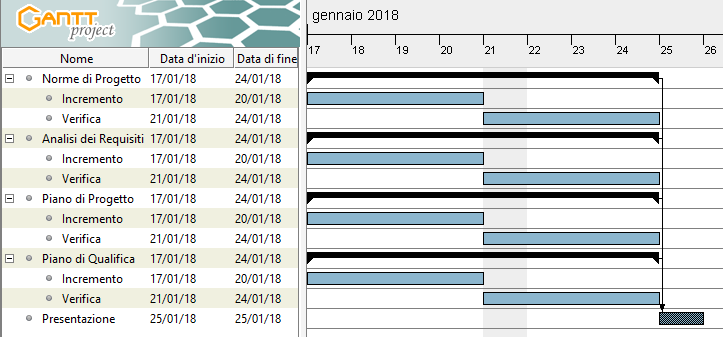
\includegraphics[width=\linewidth]{ConsolidamentoGantt.png}	
		\caption{Diagramma di Gantt di Consolidamento dei requisiti}\label{fig:2}
	\end{figure}
	\newpage
	\section{Progettazione architetturale}
	Inizia dopo la presentazione della Revisione dei Requisiti e termina il 19-03-2018 con la Revisione di Progettazione.
	Durante questa attività vengono svolte le seguenti sotto-attività:
	\begin{itemize}	
		\item \textbf{Incremento e Verifica}: vengono incrementati e verificati, se necessario, i documenti già redatti, correggendo i difetti emersi nell'esito della Revisione dei Requisiti;
		\item \textbf{Specifica Tecnica:} viene individuata l'architettura di alto livello per la realizzazione del prodotto, il documento \textit{Specifica Tecnica} contiene la descrizione dettagliata di essa;
		\item \textbf{Glossario:} vengono inseriti nuovi termini nel \textit{Glossario} e, se necessario, viene migliorato.
	\end{itemize}
	
	\subsection{Progettazione architetturale - Diagramma di Gantt}
	\begin{figure}[H]
		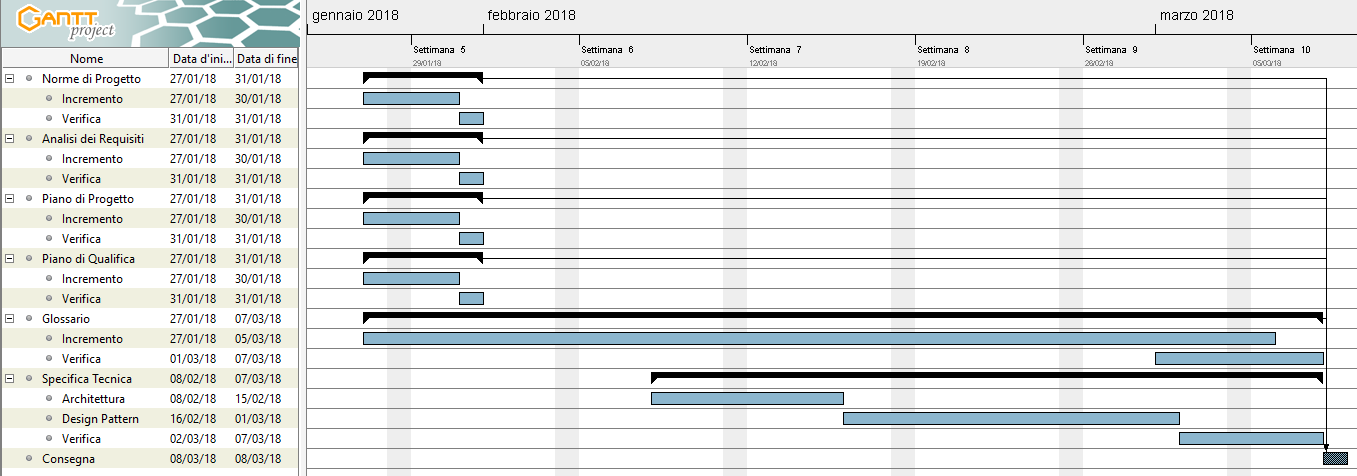
\includegraphics[width=\linewidth]{ProgArchitetturale.png}	
		\caption{Diagramma di Gantt di Progettazione architetturale}\label{fig:3}
	\end{figure}
	\newpage
	\section{Progettazione di dettaglio e Codifica}
	Inizia dopo la Revisione di Progettazione e termina con la Revisione di Qualifica del 23-04-2018. Durante questa attività vengono svolte le seguenti sotto-attività:
	\begin{itemize}
		\item \textbf{Incremento e Verifica}: vengono incrementati e verificati, se necessario, i documenti già redatti, correggendo i difetti emersi nell'esito della Revisione di Progettazione;	
		\item \textbf{Definizione di Prodotto:} viene definita nel dettaglio la struttura e il funzionamento del prodotto per la sua codifica, descrivendola nel documento \textit{Definizione di Prodotto};
		\item \textbf{Codifica:} consiste nella stesura del codice per la creazione del prodotto;
		\item \textbf{Manuale Utente:} viene redatto il documento \textit{Manuale Utente}, contente indicazioni sul corretto utilizzo del prodotto; 
		\item \textbf{Glossario:} vengono inseriti nuovi termini nel \textit{Glossario} e, se necessario, viene migliorato.
	\end{itemize}
	\subsection{Progettazione di dettaglio e Codifica - Diagramma di Gantt}
	\begin{figure}[H]
		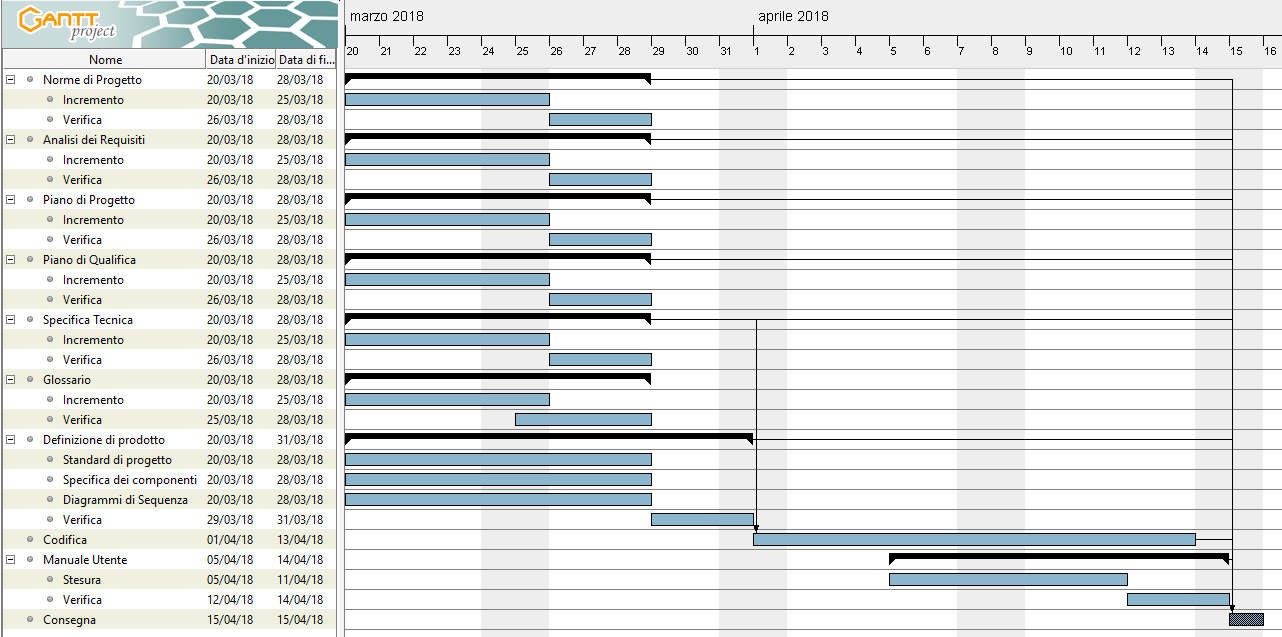
\includegraphics[width=\linewidth]{ProgCodifica.png}	
		\caption{Diagramma di Gantt di Progettazione di dettaglio e Codifica}\label{fig:4}	
	\end{figure}
	
	\section{Validazione e collaudo}
	Inizia dopo la Revisione di Qualifica e termina con la Revisione di Accettazione del 14-05-2018. Durante questa attività vengono svolte le seguenti sotto-attività:
	\begin{itemize}
		\item \textbf{Incremento e Verifica}: vengono incrementati e verificati, se necessario, i documenti già redatti, correggendo i difetti emersi nell'esito della Revisione di Qualifica;		
		\item \textbf{Validazione e Collaudo:} viene verificata la conformità del prodotto rispetto ai requisiti, testandolo per assicurarsi il corretto funzionamento ed il raggiungimento di determinati vincoli qualificativi.
		\item \textbf{Glossario:} vengono inseriti nuovi termini nel \textit{Glossario} e, se necessario, viene migliorato.
	\end{itemize}
	\subsection{Validazione e collaudo - Diagramma di Gantt}
	\begin{figure}[H]
		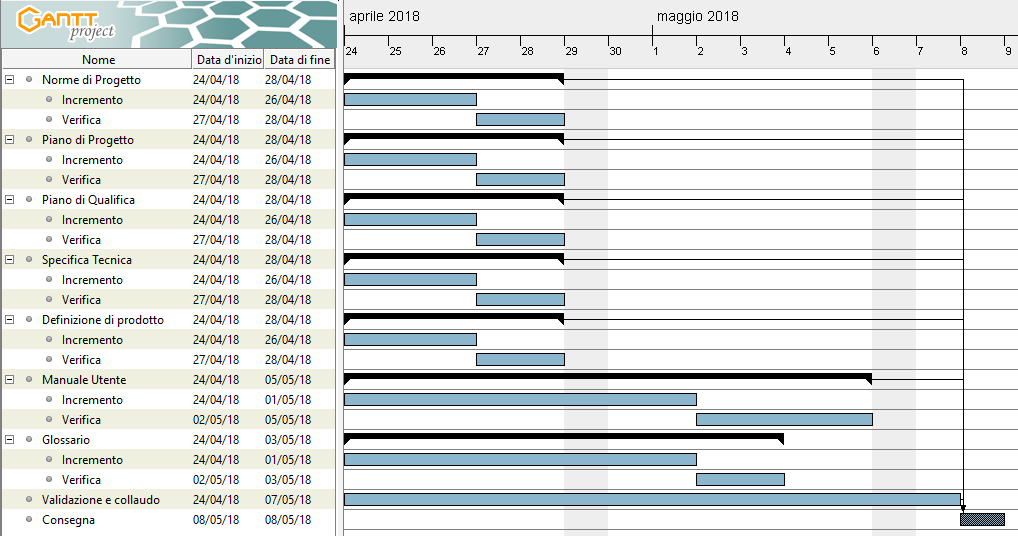
\includegraphics[width=\linewidth]{ValidazioneCollaudo.png}	
		\caption{Diagramma di Gantt di Validazione e collaudo}\label{fig:5}	
	\end{figure}
\end{document}